\setuplabframe
{Archive your lab directory}
{
  \begin{itemize}
  \item Clean up files that are easy to retrieve, remove downloads.
  \item Generate an archive of your lab directory.
  \end{itemize}
}

\ifdefempty{\evaluationformurl}{}{
\begin{frame}
  \frametitle{Evaluation form}
  Please take a few minutes to rate this training session,
  by answering our on-line survey:

  \url{\evaluationformurl}
\end{frame}
}

\begin{frame}
  \frametitle{Related documents}
  \begin{columns}
    \column{0.5\textwidth}
    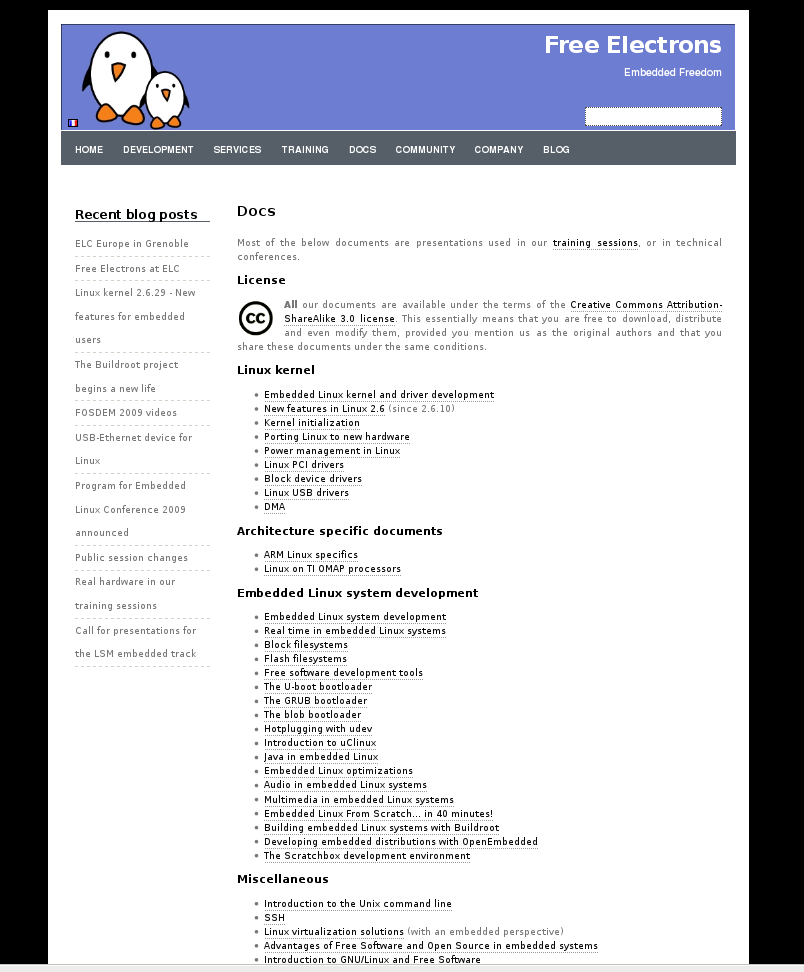
\includegraphics[width=\textwidth]{slides/last-slides/related-documents-screenshot.png}
    \column{0.5\textwidth}
    All our technical presentations on \url{http://free-electrons.com/docs}
    \begin{itemize}
    \item Linux kernel
    \item Device drivers
    \item Architecture specifics
    \item Embedded Linux system development
    \end{itemize}
  \end{columns}
\end{frame}

\begin{frame}
  \frametitle{Life after training} Here are things we could do to
  support you in your embedded Linux and kernel projects:
  \begin{itemize}
  \item BSP development for your hardware (drivers, bootloader,
    toolchain)
  \item Make the official Linux sources support your hardware
  \item System development and integration
  \item System optimization
  \item Hunting and fixing nasty bugs
  \item More training: see
    \url{http://free-electrons.com/training/}. Your colleagues who
    missed this class could go to our public sessions.
  \end{itemize}
  See \url{http://free-electrons.com/development} and
  \url{http://free-electrons.com/services}
\end{frame}

\begin{frame}
  \frametitle{Last slide}
  \begin{center}
    \Huge
    Thank you!\\
    \huge
    And may the Source be with you\\
  \end{center}
\end{frame}
